\section{Stellar Mass Completeness} \label{sec:mscomp}

First, we take galaxies with $i \Delta z < z < (i+1) \Delta z$. 

For each galaxy take their best-fit SED from {\sc PROVABGS} and artificially redshift it to 
$z' = z + \Delta z$.

afterward, calculate the $r$ band magnitude using the best-fit SED and
determine whether the galaxy at $z'$ would be within the target selection. 


We then compare the $M_*$ distributions and determine the $M_*$ below which  a
significant number of galaxies are excluded from the sample.  


\begin{figure}
\begin{center}
    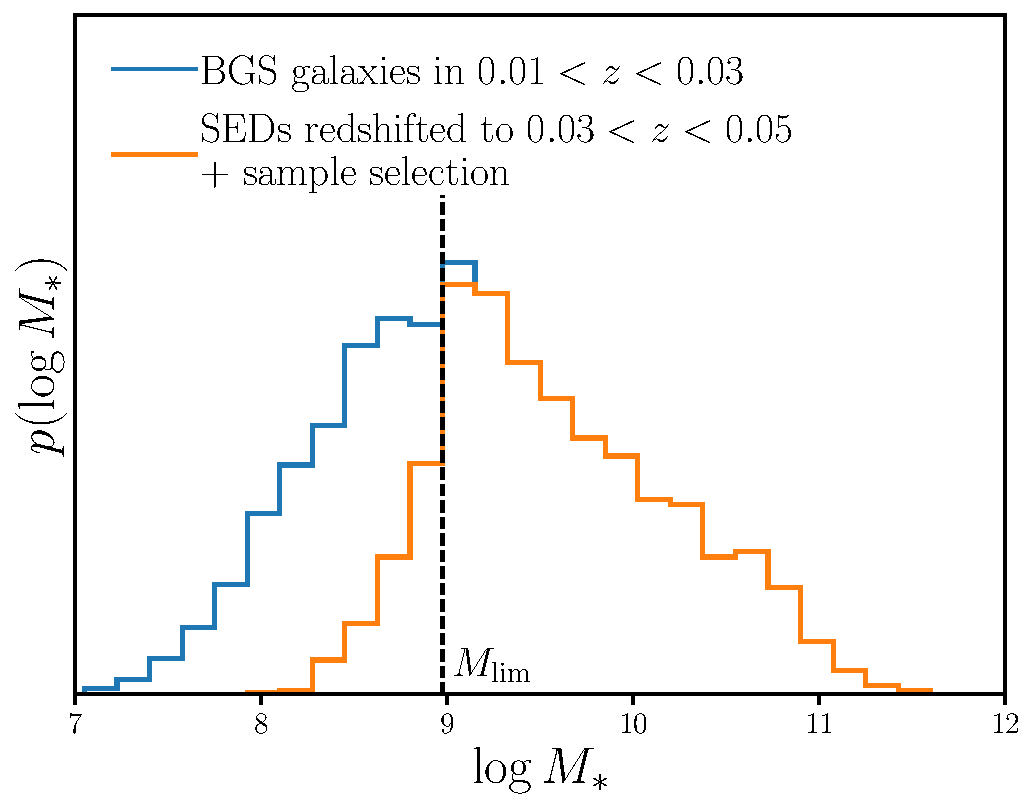
\includegraphics[width=0.45\textwidth]{figs/psmf_logMstar_comp_demo.pdf}
    \caption{blah
    }\label{fig:ms_comp0}
\end{center}
\end{figure}
%\begin{figure}
%\begin{center}
%    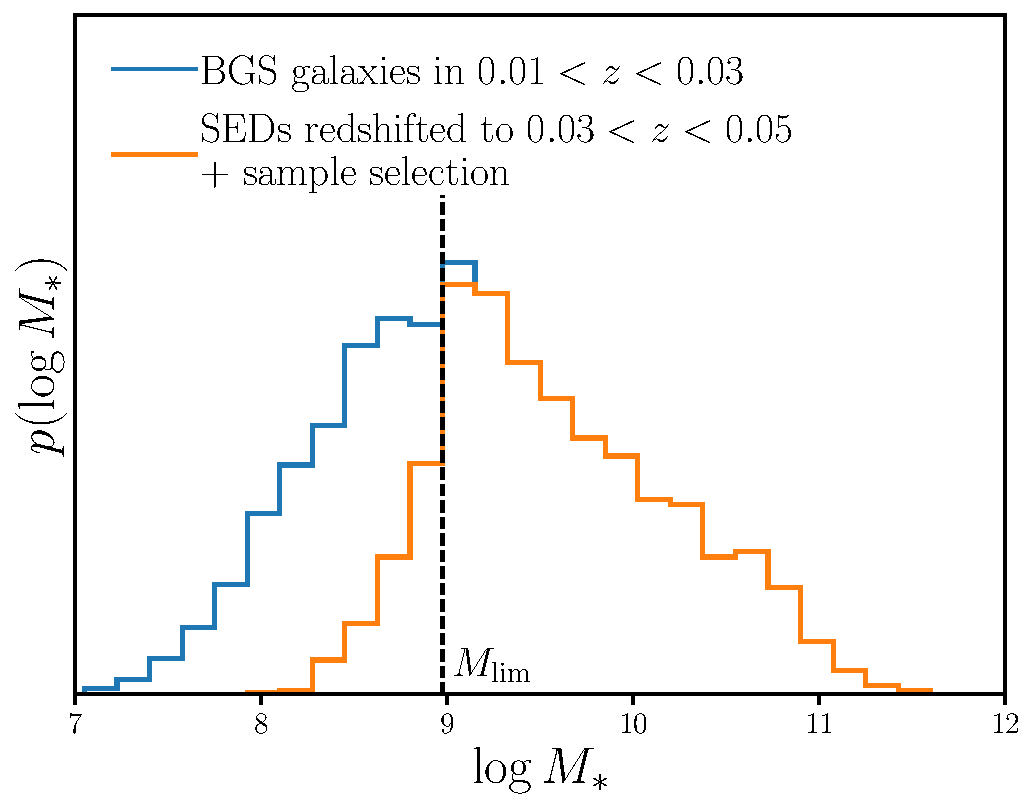
\includegraphics[width=0.5\textwidth]{figs/psmf_logMstar_comp_demo.pdf}
%    \caption{
%        To determine the $M_{\rm lim}$, the $M_*$ completeness limit, we
%        galaxies in redshift bin
%    }\label{fig:ms_comp0}
%\end{center}
%\end{figure}


%\begin{figure}
%\begin{center}
%    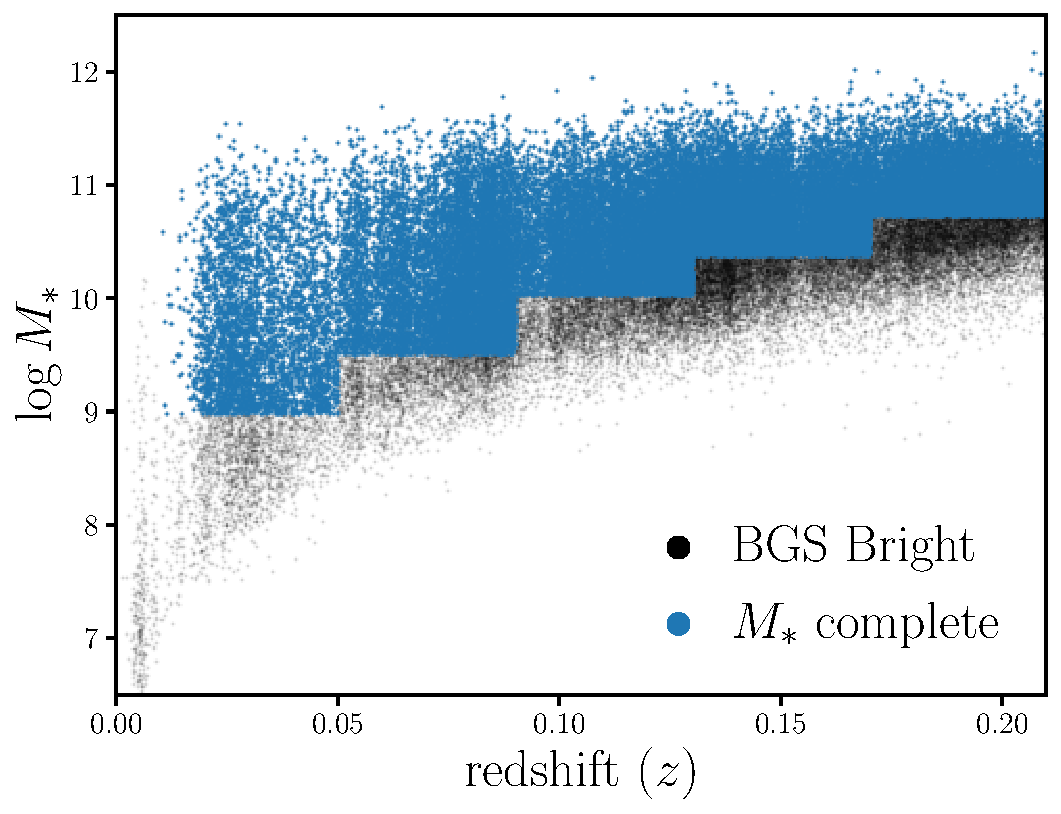
\includegraphics[width=0.6\textwidth]{figs/psmf_logMstar_comp_z.pdf}
%    \caption{
%    }\label{fig:ms_comp1}
%\end{center}
%\end{figure}
